\documentclass{article}
\usepackage{apacite}
\usepackage{graphicx}

\title{Sample Size Calculation for a SARS-Cov-2 Serological Test Validation Study}
\author{Enveritas}

\begin{document}
\nocite{*}
\maketitle
\bibliographystyle{apacite}

\begin{figure}
  \centering
  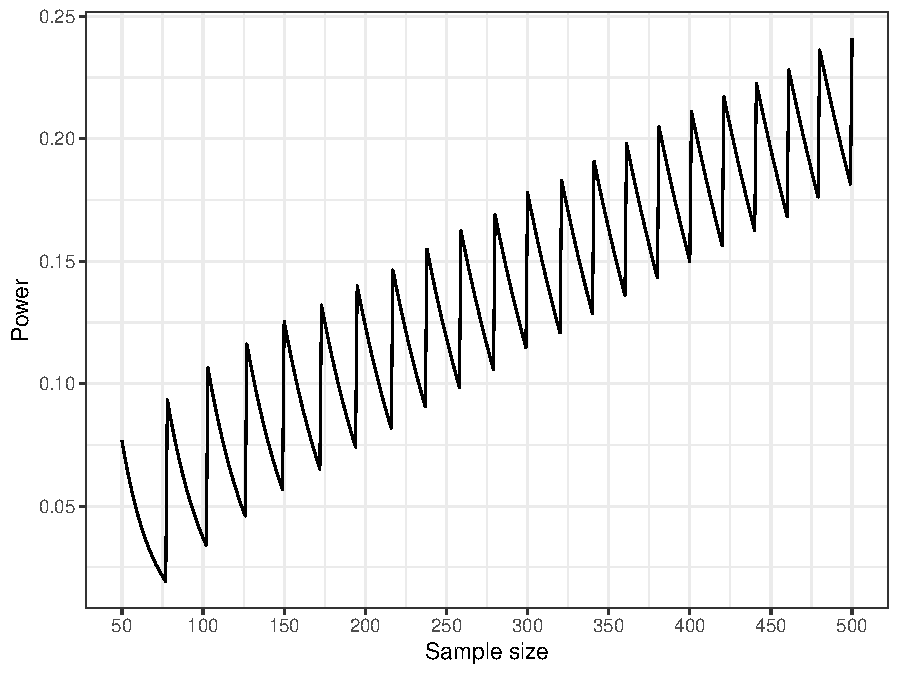
\includegraphics[width=\linewidth]{img/power_saw.pdf}
  \caption{power as function of increasing sample size does not increase monotonically }
  \label{fig:power_saw}
\end{figure}


\begin{figure}
  \centering
  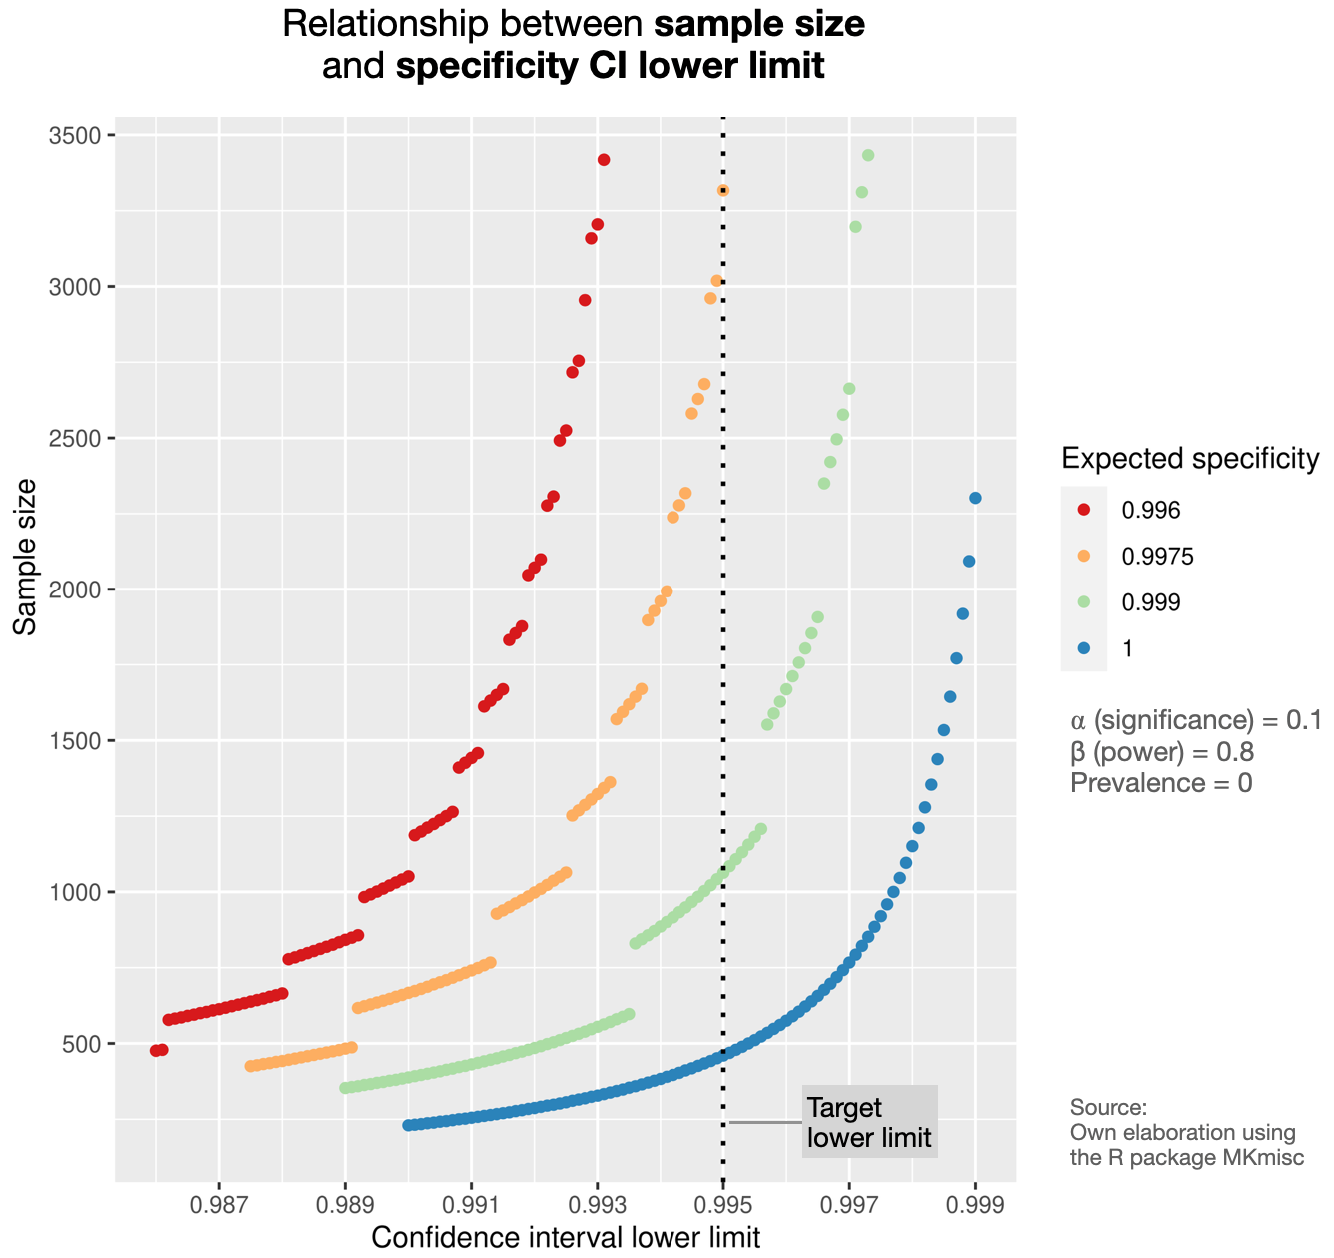
\includegraphics[width=\linewidth]{img/editedByHand_sample_size_sp_lim.png}
  \caption{lim vs ss}
  \label{fig:lim_vs_ss}
\end{figure}



We need exact methods because the normal approximation is not accurate at our typical required sample size (between 150 and 250 patients) when the  efficacy parameter is expected to be 0.95 or higher. This is particularly serious because the comparison of exact methods with normal approximations generally shows that the normal approximation significantly underestimates the required sample size in these situations. So not only is it inaccurate but it also errs in precisely the wrong direction!

Diagnostic tests are typically associated with very high values of sensitivity and specificity. In such cases, sample size calculation based on a normal approximation to the binomial distribution may be misleading. With modern computing, it is feasible to replace normal approximations with exact methods.\cite{chu2007sample}

for tests of a single binomial proportion compared to a hypothesized standard, statistical power does not monotonically increase as a function of increasing sample size: the power function appears to be ‘‘saw toothed’’\cite{chu2007sample}

To evaluate the accuracy of specificity estimate, the experimenter must further estimate some confidence limit. The $1-\alpha$ lower confidence limit for Sp can be thought of as the lowest value of Sp that is not rejected by a one-sided test of level $\alpha$ of the null hypothesis $Sp = Sp_L$ against the alternative hypothesis $Sp > Sp_L$. Upper con fidence limits are defined in an analogous manner, but are irrelevant here, because the concern is that the test actually performs worse, not better, than indicated by the observed proportion of positive outcomes in the trial sample.\cite{flahault2005sample}. The normal approximation is eplained in \cite{machin1997sample} and \cite{hajian2014sample}.

\begin{equation}
N = \frac{\left(z_{1-\alpha/2}\sqrt{\pi_{1}\left(1-\pi_{1}\right)} + z_{1-\beta}\sqrt{\pi_{2}\left(1-\pi_{2}\right)} \right)^2}{\delta^2}
\end{equation}

one sided test (tail), reordering and setting $\pi_{1}=\pi - \delta$ and $\pi_{2}=\pi$:
\begin{equation}
  \label{eq:normalaprox}
N = \frac{\left(z_{1-\beta}\sqrt{\pi\left(1-\pi\right)} + z_{1-\alpha}\sqrt{\left(\pi - \delta\right)\left(1-\pi+\delta\right)} \right)^2}{\delta^2}
\end{equation}

\begin{equation}
\sum_{i = x}^n {n\choose i}\hat{\pi}_L^i(1 - \hat{\pi}_L)^{n-i} = \alpha
\end{equation}

\begin{equation}
\sum_{i = q_{\beta}}^n {n\choose i}\gamma^i(1 - \gamma)^{n-i} = \alpha
\end{equation}

\bibliography{References}
\end{document}
